\documentclass[twocolumn]{article}

\usepackage{amstext}
\usepackage{amsmath}
\usepackage{graphicx}
\usepackage{float}
\usepackage{caption}
\usepackage{subcaption}
\usepackage[margin=1in, paperwidth=8.5in, paperheight=11in]{geometry}
%\usepackage{gensymb}
\usepackage{here}
\usepackage{caption}

\usepackage[backend=biber]{biblatex}
\addbibresource{references.bib}

\def\changemargin#1#2{\list{}{\rightmargin#1\leftmargin#2}\item[]}
\let\endchangemargin=\endlist
\begin{document}

\title{Wolbachia, Toxoplasma and O. Cordyceps: Extreme Host-Manipulating Microbes That Are Changing the World}
    \author{C. Bekins, R. Chapman and B. Wasti}
    \date{December 2015}
    \maketitle

\section*{Introduction}
When thinking of infection most people will think of getting sick or of a swelling cut that is turning green. However, most people do not think about wandering around randomly and trying to climb a tree, only to have a fungus grow out of their spinal column. That is because humans are (mostly) lucky with respect to infections in this world; the worst we have to worry about is dying.

For other animals, dying is possibly the best case for an infection. There are a few microbes that will manipulate their host to extreme lengths. From hijacking the reproductive systems to complete mind control, and seemingly everything in between, the parasitic microbial world has developed a whole range of tools for which to survive at any cost. In this paper, we will go over three of these host-manipulating microbes, each with a different characteristic: \textit{Wolbachia}, the reproductive-system hijacker; \textit{Toxoplasma}, the subtle schizophrenic inducer; and the infamous \textit{O. Cordyceps}, the mind-controlling fungus. 

\section*{Wolbachia}
\textit{Wolbachia} is a group of bacteria that infects arthropod species. Technically there is only one true type of \textit{Wolbachia}, \textit{Wolbachia pipientis}, but due to the genetic diversity of different strains, it is commonly split into two groups, group A and group B, although it is generally just referred to as \textit{Wolbachia}.

The bacteria is found in the ovaries and testes of a wide range of arthropods.\cite{Wbio} It is passed on via reproduction, and can only be spread through females. \textit{Wolbachia} are considered mutualistic endosymbionts, and are ``required for survival of their hosts."\cite{Wdisc_nem} An interesting thing to note is how universal \textit{Wolbachia}seems to be. It has been demonstrated that \textit{Wolbachia} infects 25-70\% of species of insects.\cite{Wdisc_nem}

To give a bit of background,\textit{Wolbachia} was first discovered by Samuel Burt Wolbach and described by Marshall Hertig in 1924.\cite{Winit} Wolbach had been studying the cause of Rocky Mountain Spotted Fever and by 1916 had shown that \textit{Dermacentor andersoni}, a tick native to the Rocky Mountain area, was the transmitter of the disease.\cite{wolbachia} He was unable to grow the actual bacteria causing the disease, a species of \textit{Rickettsia}, in a cell-free culture leading ``him to speculate as to the relationship between the cells of the host and the intracellular parasites."\cite{wolbachia} This is important to note, because the discovery of \textit{Wolbachia} is closely linked to this idea.

\begin{figure}[!ht]
    \centering
    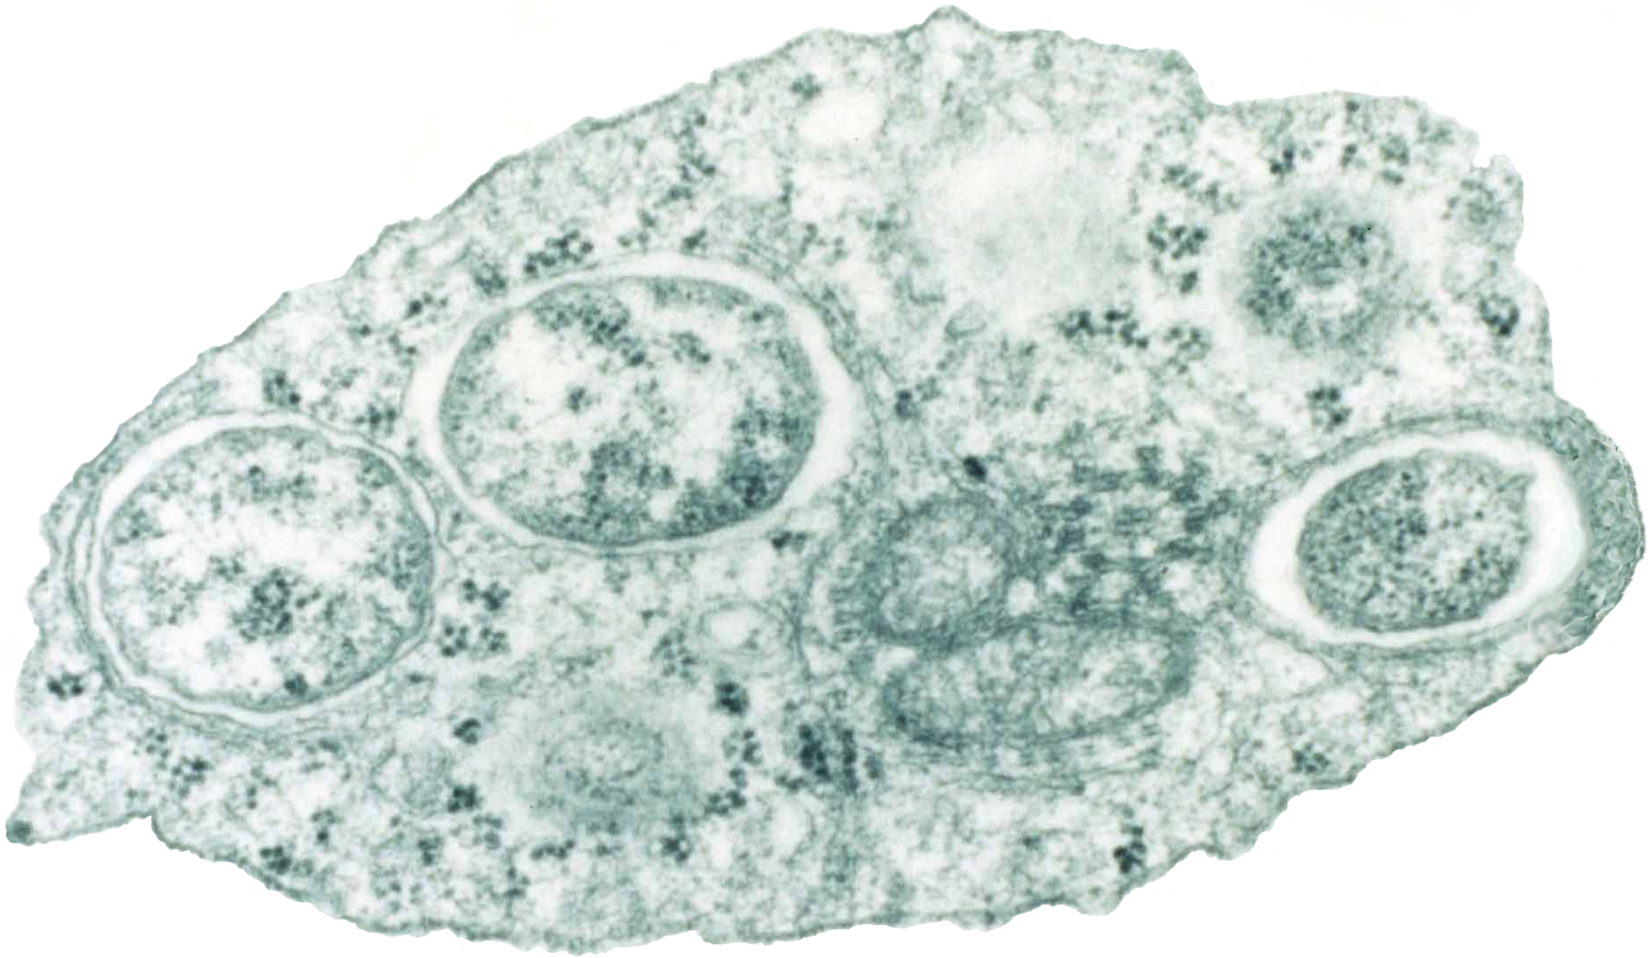
\includegraphics[width=.4\textwidth]{images/Wolbachia.png}
    \caption{\textit{Wolbachia} bacteria (Green circles) inside a host cell. It is difficult to tell that there is a bacteria present if one is unaware.\cite{Wwiki_image} }
    \label{fig:wolbachiha_tree}
\end{figure}

Hertig came to work with Wolbach, and together they investigated a bacteria living in the gonads of the \textit{C. pipiens} mosquito. This bacteria is known today as \textit{Wolbachia pipientis} which Hertig gave a detailed description of in 1936.\cite{Wdiscription} At this point scientists did not know of the gene manipulation that \textit{Wolbachia} has on it's hosts, and the discovery largely went unnoticed.

During the 1950s a group of scientists found that certain matching between \textit{Culex} mosquitos produced no offspring. They named this phenomenon cytoplasmic incompatibility, although they were not sure as to what the cause was.\cite{Wcyto_iso} It wasn't until the 1970s that cytoplasmic incompatibility was linked to \textit{Wolbachia}, when a group of scientists eliminated the \textit{Wolbachia} through antibiotics.\cite{Wcyto_cause}

Also during the 1960s and '70s scientists noted ``unusual structures in the oocytes or in the hypodermis" of filarial nematodes but did not associate them with bacteria.\cite{wolbachia} It wasn't until 1995 that these ``unusual structures" were determined to be \textit{Wolbachia}.\cite{Wstruct} 

The history of \textit{Wolbachia} is rather curious, and for good reason. On the surface, \textit{Wolbachia} are just harmless bacteria living in the reproductive areas of different insects that don't really do anything. But only recently has it been shown that \textit{Wolbachia} has shaped the world in drastic ways, and is one of the most prolific parasitic bacteria.\cite{Wdistr}

There is a very good reason for the abundance of \textit{Wolbachia}, for better or for worse, it completely hijacks the host organism's reproductive organs. One of the most unique features of \textit{Wolbachia} is the reproductive changes it makes in its host species. It can cause cytoplasmic incompatibility \cite{Wci0}\cite{Wci1}\cite{Wci2}\cite{Wci3}, parthenogenesis \cite{Wparth}, feminization of males \cite{Wfem} and male killing.\cite{Wmale_killing} All of these different changes force the host species to pass on \textit{Wolbachia} to their offspring, also known as vertical transfer.

%##### How does it function?
The most prominent of these reproductive changes is cytoplasmic incompatibility which is a ``reproductive incompatibility between sperm and egg."\cite{Wbio} \textit{Wolbachia} can only be passed on through eggs, and not sperm, so in order to get around this limitation it has evolved to not allow inter-breeding between members of the same species where only one of them is infected with \textit{Wolbachia}. However, it gets even more complicated than this.

There are actually two types of cytoplasmic incompatibility, unidirectional and bidirectional. Unidirectional allows an infected female to mate with an uninfected male, which makes sense because the \textit{Wolbachia} can still be passed on. Bidirectional cytoplasmic incompatibility occurs when there is no case where an infected member and an uninfected member can mate succesfuly. The reason for these two different 'modes' is even more complicated still.

It goes back to the idea that there are two separate groups of \textit{Wolbachia}, group A and group B. Comparing the 16S rDNA does not give a full picture for the genetic diversity of the \textit{Wolbachia}, and the ftsZ gene was used to compare the genetics of 38 different \textit{Wolbachia} strains.\cite{Wgenetics} It was found that there is in fact a very large genetic difference between strains, and that group A and group B diverged 58-67 million years ago. Figure \ref{fig:wolbachia_tree} shows a part of the tree for the strain distribution of Wolbachia.

\begin{figure}[!ht]
    \centering
    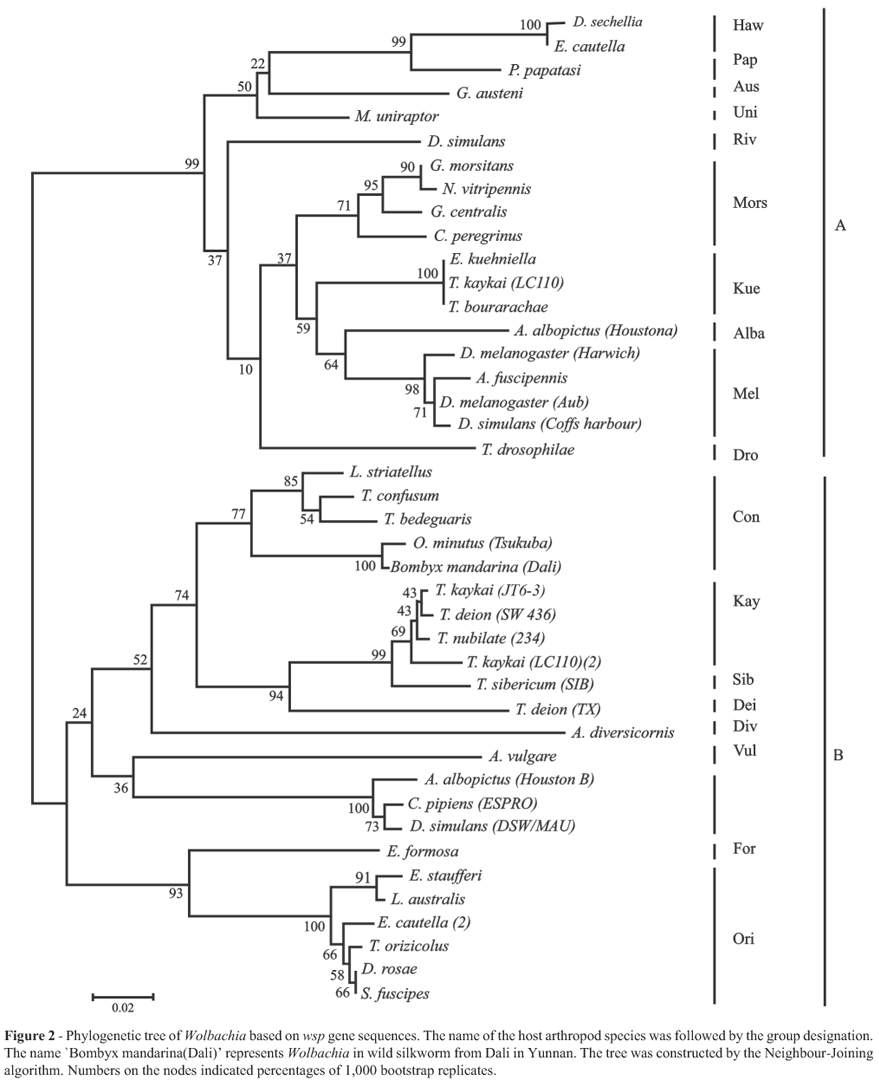
\includegraphics[width=.4\textwidth]{images/WolbachiaTree.jpg}
    \caption{ A depiction of the strain distribution for Wolbachia. Most importantly, the separation between group A and group B is depicted. \cite{Wtree_image} }
    \label{fig:wolbachia_tree}
\end{figure}

Going back to cytoplasmic incompatibility, when a species is infected with two different strains of \textit{Wolbachia} (a species can in fact be infected with multiple strains) that are mutually incompatible, bidirectional cytoplasmic incompatibility occurs.\cite{WbiCI} It makes more sense when discussing how \textit{Wolbachia} cause this cytoplasmic incompatibility.

The exact mechanisms for the cause of cytoplasmic incompatibility are not known. What is known is that the \textit{Wolbachia} in the male modify the sperm in such a way that only if the same strain of \textit{Wolbachia} is in the female species to ``recover" the sperm will correct fertilization occur.\cite{Wbio}

In many ways \textit{Wolbachia} acts like an encryption algorithm, ``encrypting" the sperm sent to the female, and only if the female has the correct decryption algorithm can she get pregnant. This is also why different strains of \textit{Wolbachia} are incompatible, using a wrong decryption algorithm will generate nonsense.

The other unique reproductive change \textit{Wolbachia} causes is parthogenisis, or the ability for unfertilized eggs to grow into healthy adults essentially eliminating the need for males in a species. This makes sense, \textit{Wolbachia} can only be passed on through females, so it does not care about the males. But then one might realize that \textit{Wolbachia} took over the male's job, and took millions of years of evolution for sexual differentiation and threw it out the window.

Perhaps the most famous case of parthogenisis caused by \textit{Wolbachia} is in the \textit{Trichogramma} wasps, where all members of the species are female. Weirdly, by treating the wasps with antibiotics to kill of the \textit{Wolbachia} cause ``some female parthenogenetic strains ... to revert to production of male progeny."\cite{Wpar_removal} It would appear that \textit{Wolbachia} is merely surpressing the need for male's in certain species. Even stranger is the fact that ``phylogenetic evidence suggests that [parthogenisis] has evolved several times independently in these bacteria" which, as one scientist puts it, suggests ``a simple biochemical mechanism."\cite{Wbio}  

Despite the fact that we still do not know the exact biochemical mechanism that causes parthogenisis, we do know that it is the result of gamete duplication.\cite{Wgamete_duplication} There is still work to be done in order to figure out how \textit{Wolbachia} is inducing gamete duplication.

In fact, there is a lot of research that needs to be done on \textit{Wolbachia} in general. There is still so much that is not known about the bacteria, even how many organisms it infects is a mystery. However, there is another microbe which might be even more mysterious than the \textit{Wolbachia}.

\section*{Toxoplasma}
\textit{Toxoplasma gondii} is a “coccidian parasite of cats with all non-feline warm blooded animals (including humans) as intermediate hosts” \cite{Tlife_cycle}. It was first discovered by scientists in 1908 in the rodent Ctenodactylus gundi, known commonly as the North African Gundi \cite{Tlife_cycle}. In 1917, it was discovered that gundis were not infected naturally, but through life in captivity. This raised the question of transmission, and transmission remained mysterious for years, as scientists tried again and again to understand it but came up with “essentially unsuccessful results” \cite{Tlife_cycle}. Now, thanks to the work of several scientists between the 1960s and late 1990s, we understand that \textit{T. gondii} is generally contracted by the ingestion of infected meat or through contact with cat faeces \cite{Tlife_cycle}. We also have begun looking into transmission via birds, which was not initially considered because all other hosts thus far discovered have been mammals \cite{Tbirds}, and the mechanics behind how dogs might transfer the bacteria from cat faeces to humans \cite{Tdogs}.

We also understand now that \textit{T. gondii} infects and reproduces sexually within cats, but all other mammals can also carry the bacteria and become affected by it. Once \textit{Toxoplasma gondii} has entered the body, it makes its way to the lining of the intestines. There, it begins to replicate. In non-feline mammals such as mice, the bacteria reproduces asexually and begins to move throughout the body. Migration into the bloodstream allows the bacteria to reach all parts of the body, including soft tissue, the lymph nodes, and the brain. Tissue cysts begin to form and \textit{T. gondii} continues to replicate \cite{Tmice}. In cats, \textit{T. gondii} reproduces sexually and its oocysts are shed by the cat in its feces. Transmission of these oocysts from the feces to other mammals, either via direct contact or some proxy, is what allows the bacteria to infect its intermediate hosts. Strangely enough, cats have shown signs of immunity to this shedding. Cats do not appear to be negatively affected by \textit{T. gondii's} presence, however there is evidence that a cat which has shed oocysts once has an immunity to shedding them again \cite{Tcat_immunity}. A study was done to test whether or not this immunity lasts for 6 years, and it in fact appears to, unless the cat comes into contact with a more virulent strain of \textit{T. gondii} \cite{Tcat_immunity}. This is an intriguing phenomenon – how can \textit{T. gondii} be effectively spread if cats no longer shed its oocysts after having been infected just once? And why do cats develop this immunity if they are not negatively affected by the bacteria?

Regardless, \textit{Toxoplasma gondii} is spread and its cycle does appear to be effective. \textit{T. gondii's} most common modus operandi is to infect rats and make the rats a tool for re-infecting cats. Rats that are infected by \textit{T. gondii} have been studied and observed to be “significantly more active than their uninfected counterparts,” while rats infected with other parasites that also have life cycles similar to that of \textit{T. gondii} did not show any altered behavior \cite{Trat}. Although “the mechanism of action by which \textit{T. gondii} alters rodent behavior is unknown” \cite{Trat}, this does show that rodent behavior is affected by \textit{Toxoplasma gondii}. The current understanding is that infected rats become more active (and therefore more available to cats), while simultaneously losing their aversion to the smells associated with cats \cite{Tpodcast_replace}. Rats then become easy targets, so cats eat them and the tissue cysts formed by \textit{T. gondii} travel to the cat’s intestines, where the cycle begins again.

\section*{Cordyceps}
Cordyceps, or more specifically \textit{Ophiocordyceps unilateralis}, is a fungus that infects ants. Otherwise known as a specialized fungal parasite. This zombifying, mind-controlling microbe is able to modify the behavior of its host. Eventually it kills its host in a location optimal for its reproduction. 

The story of how \textit{Ophiocordyceps} functions is a cycle, so you could start talking about it anywhere, but from an ant's perspective everything starts when it comes into contact with the spores of the fungus. The spores recognize they are on a host, and form a biological drill that utilizes enzymes and mechanical pressure to breach the ant's tough exoskeleton. Once inside, the fungus transforms into a yeast-like state, living in the hemocoel of the ant.\cite{cordy_infection} This is where the highly specialized adaptations of \textit{Ophiocordyceps} start to shine. There are many things that are unknown about how \textit{Ophiocordyceps} manipulates the mind of its host, but the outcome has been studied in depth. \textit{Ophiocordyceps} leads its host ant to the northern side of a sapling approximately 25 cm above the ground. There, the ant closes it mandibles on the bark of the sapling or the main vein on the bottom side of a leaf, never to open them again. It is there that the fungus rapidly colonizes the host, restructuring all nutrients available inside the host to produce a large fruiting body which grows out of the back of the ants head that will produce the spores to restart the cycle.\cite{life_of_dead_ant}

\begin{figure}[!ht]
    \centering
    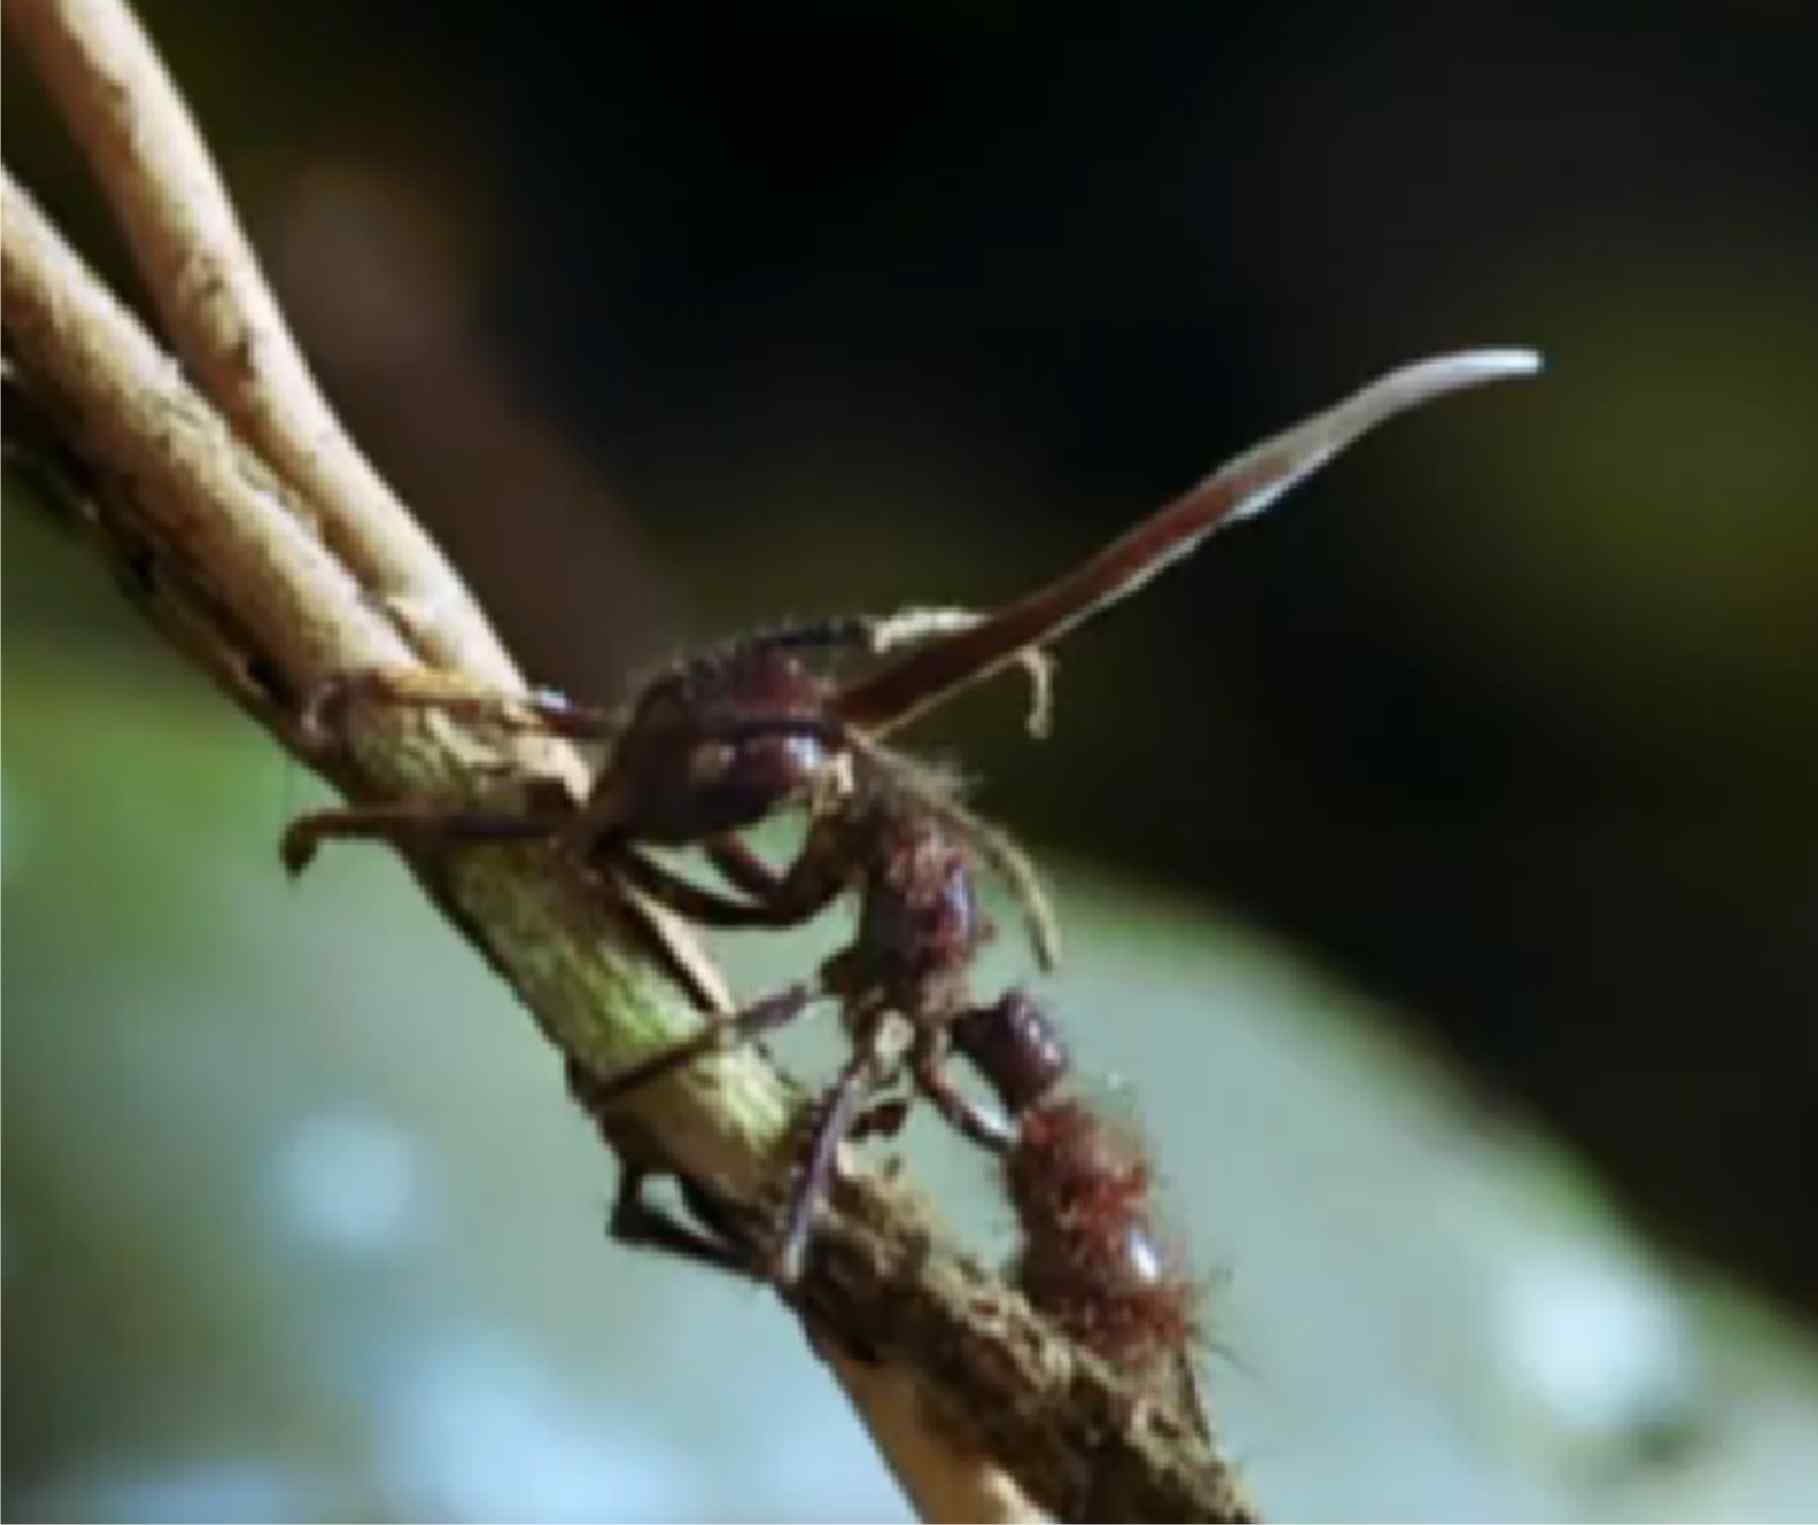
\includegraphics[width=.4\textwidth]{images/cordyceps_ant.jpg}
    \caption{The spore bearing fruiting body of \textit{Ophiocordyceps unilateralis} growing out of the back of the head of an ant whose mandibles are tightly gripping a twig.\cite{cordy_video} }
    \label{fig:cordyceps_ant}
\end{figure}

\textit{Ophiocordyceps unilateralis} was first discovered in 1859 by the British naturalist Alfred Russel Wallace who, probably not coincidently, is best known for independently conceiving the theory of evolution through natural selection. Darwin published his now famous ``On the Origin of Species" in the same year, which gives some good context as to where the scientific paradigms were at the time.\cite{darwin} 

\section*{Impacts And Analysis}

Scientists have only recently begun doing research on the three microbes discussed above. However, the three microbes mentioned have had a massive impact on the world as we know it. 

A cousin of the ant manipulating fungus, \textit{Cordyceps sinensis} has been a cornerstone of Chinese medicine for centuries. It has been claimed it can be used to treat many things including respiration and pulmonary diseases, renal, liver, and cardiovascular diseases, hypo sexuality, and hyperlipidemia. Most of these purported benefits have yet to be sufficiently investigated since interest from the western world only began to increase in the last two decades. \cite{medicinal_cordy} Another Cordyceps species, \textit{Cordyceps subsessilus} was used to create the immunosuppresive drug cyclosporin, which is widely used in organ transplantation. The drug prevents the rejection of the foreign organ by interfering with the growth of T cells and the activity of the immune system.\cite{cordy_tcells}

The parasitic Cordyceps fungi are key to the diversity of the ecosystems they live in. If any one population of insects begins to become dominant in the ecosystem, it becomes an easy target for a Cordyceps fungus to infect.  \cite{cordy_video}

\textit{Toxoplasma gondii} is a microbe that we may have only discovered 107 years ago, and most people have never heard of it, but it still has a large impact on the human population. ``Infection with \textit{Toxoplasma gondii} can cause severe illness when the organism is contracted congenitally or when it is reactivated in immune-suppressed persons” \cite{Tsero}, which is how it most greatly affects people. Many people afflicted by AIDS or cancer have developed toxoplasmosis due to the weakened state of their immune systems. Children are also at risk for serious complications caused by \textit{T. gondii}, as exemplified by the fact that when research into this microbe began, one of the first examined victims was an infant girl who died at one month old due to congenital toxoplasmosis \cite{Tlife_cycle}.

Humans infected by \textit{T. gondii} can exhibit a variety of symptoms. Most people are not at all aware of their infection. Some experience flu-like symptoms, including swollen lymph nodes and muscle aches. However, serious cases can lead to infections in the eyes, brain, and other organs. Some infants infected congenitally are born with serious eye or brain damage, and others who may not have symptoms right away may develop them later in life \cite{Tsymptoms}. In addition, there is research suggesting that people who own cats during childhood may be more likely to be diagnosed with schizophrenia later in life \cite{Tschiz}. The full impacts of \textit{Toxoplasma gondii} on humans have yet to be quantified and understood, but the impacts of which we are currently aware are substantial.

Let’s not forget that \textit{Toxoplasma gondii} is found everywhere. Birds carry it and can shed the oocysts, spreading the microbe \cite{Tbirds}. There is speculation that dogs might carry it on their fur and aid in the transmission of the microbe to humans \cite{Tdogs}. And scientists have come to believe that ``some 25 percent of the global human population is chronically infected with T. gondii” \cite{TUSDA}. Currently, there is no vaccine that is safe for humans to use against \textit{T. gondii} \cite{Tvaccine}, but research is continuing, particularly at the Toxoplasmosis Research Institute and Center in Chicago, IL. This microbe may have bigger plans for us than we can even imagine at this point, so research into it should continue until we understand it better.

The presence of \textit{Wolbachia} in filarial nematodes has raised interesting questions about how \textit{Wolbachia} evolves in its host species. Some scientists discovered that \textit{Wolbachia} ``have possibly been lost during evolution along some lineages of filarial nematodes."\cite{Wevolution_loss} The reason this discovery is bizare is because \textit{Wolbachia}'s ability to evolve into the life-cycles of so many different species makes sense if \textit{Wolbachia} gives the infected a fitness advantage over uninfected members. However, if species evolve to get rid of \textit{Wolbachia} then this points to the fact that \textit{Wolbachia} does not supply them with a fitness advantage.

So why would one species derive an advantage from a \textit{Wolbachia} infection whereas another species might not? The answer is that nobody really knows, at least not yet. The impact this discovery has had on our understanding of evolution has not truly been felt yet. However, when the reason for differences in derived fitness advantage from \textit{Wolbachia} infections is understood it could uncover a greater understanding of how interactions between organic matter works. It might explain why some people like coffee and find it helps them get work done, while others do not even like the smell of coffee.

Aside from helping us understand the world better, \textit{Wolbachia} may have the ability to help cure humans of deadly diseases. A recent study found that \textit{Aedes aegypti} mosquitos infected with \textit{Wolbachia} cause it to no longer be able to carry the pathogen that causes Dengue Fever.\cite{Wdengue_fever}

This is big news, because it might lead to the eradication of Dengue Fever, for which there is currently no vaccine. By artificially bringing \textit{Wolbachia} into the \textit{Aedes aegypti} species the fear of Dengue Fever could vanish entirely. Not only does this impact those in Dengue Fever risk areas, but it may also lead to the prevention of other diseases as well. Many scientists are looking into the idea of infecting mosquitos that harbor \textit{Milaria} with \textit{Wolbachia} as a prevention technique.\cite{Wmilaria}

Using \textit{Wolbachia} as an ``antidote" for different diseases is novel and has potential to change the world dramatically. The best part is that it is a one-time use antidote, because \textit{Wolbachia} has the tools to infect an entire species through vertical transmission. It may also cause scientists to look at other symbiotic relationships between organisms, and see if they have any potential to help humans. There might be a new era of using living organisms as tools to cure diseases and help humans in other ways.

The abuse of the relationship between \textit{Wolbachia} and its host may also be done in the opposite way. A species infected with \textit{Wolbachia} becomes dependant on \textit{Wolbachia}. If the \textit{Wolbachia} were to be killed off, say by antibiotics, then the host would struggle to survive. This idea can be used to treat filarial infections in humans: targetting the \textit{Wolbachia} kills off the filaraea.\cite{wolbachia}\cite{Wcure_filarial_infection}

Although this technique is rather new and is not widely used yet, it has potential to be a whole new route by which we can treat filarial infections. By combining antiwolbachia medication with antifilarial treatments, there is twice the potential to successfully cure the infection. Through studying \textit{Wolbachia}, we can save lives.


\section*{The Efficacy of Adding These Microbes to the Six Microbes Class Syllabus}

As great as the three microbes mentioned above are, they are not the ideal candidate for addition to the Six Microbes Class Syllabus. Scientifically there is still so much more to be learned about them, and there is really not much that can be done in a laboratory setting that involves these microbes and is safe or legal. These microbes have been around for a long time, but only recently has research been done on them. They just have not been around long enough to have had an impact yet.

These microbes are incredibly unique, and have awesome characteristics in terms of science. Mind-control and reproductive system hijacking not only sounds awesome, it is awesome. However, the actual details of how these microbes do what they do is still unknown. The general idea is there, but the in-depth analysis of the exact chemical process is not. For now, these microbes have \textit{awesome} characteristics, but there is so much more to learn about them that the science is a little lacking.

Although it would be really enjoyable to watch \textit{Cordyceps} fungii growing out of an ant’s skull, it would not make the most active laboratory study. \textit{Wolbachia} may not be the best idea because bringing a bunch of wasps into a small, enclosed lab room has a lot of potential for things to go wrong. Likewise, infecting students with \textit{Toxoplasma} to test if they develop schizophrenia would be interesting -- although possibly not legal. In general, these microbes do not lend themselves easily towards laboratory studies, especially ones that are meant to be conducted over one or two weeks. 

The oldest evidence that we have of the \textit{Cordyceps} fungus influencing the mind of ants are some fossilized leaves with the distinct marks of the signature “death grip” on them. Radiometric dating of the fossils shows that they are approximately 47 millions years old, making them the oldest known record of behavioral manipulation.\cite{old_leaf}

Despite having evolved behavioral manipulation abilities so long ago, the fungi have not particularly expanded their impact on the world. 47 million years ago the closest animal to a human on earth was a group of dry-nosed monkeys. 

Like the \textit{Cordyceps}, the \textit{Wolbachia} and \textit{Toxoplasma} have been around for a while, although scientists do not know for sure if they have changed all that much. In general, all three microbes have not had much of a historical impact on humans. There are no mind controlled humans that can be linked to either \textit{Toxoplasma} or \textit{Cordyceps}, and as far as we know there is no \textit{Wolbachia} living inside of us. The impacts have yet to be historical for these microbes, and in fact they only exist in the future.


    Although these microbes have had a massive impact on how life has developed, they have not yet had a massive impact on human life (at least that we can describe). However, these microbes are really only just beginning to be researched, and the potential they bring for changing the world is very high. From curing diseases and making medicine to helping us understand evolution, these microbes \textit{will} change the world. We just have not been studying them long enough to know \textit{how} just yet.


\printbibliography

\end{document}
